\newpage
\hypertarget{m2tvis}{}
\subsection{Polishing the TGG Transformation}
\visHeader

\begin{itemize}

\item[$\blacktriangleright$] Return to EA and open the \texttt{NodeToDictionaryRule} diagram, and add a constraint to \texttt{dictionaryNode} as depicted in
Fig.~\ref{ea:NodeToDictionaryRuleUpdated}.

\vspace{0.5cm}

\begin{figure}[htp]
 \hspace{-1.5cm}
  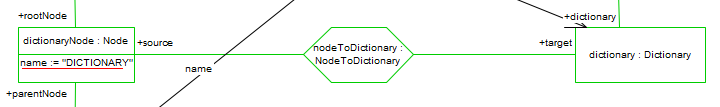
\includegraphics[width=1.2\textwidth]{ea_NodeToDictionaryRuleUpdated}
  \caption{updated NodeToDictionary}
  \label{ea:NodeToDictionaryRuleUpdated}
\end{figure}

\item[$\blacktriangleright$] Similarly, open the \texttt{ForAllEntryRule}. Add a \texttt{``ENTRY''} constraint to \texttt{entryNode}, and add a new
\texttt{setDefaultNumber} constraint by pressing \texttt{Add} in the TGG constraint dialogue window, and completing each field as shown in
Fig.~\ref{ea:setDefaultConstraintDialogue}.\footnote{ To review the purpose of constraints and discuss the significance of each of the attribute options, refer
to Part IV, Section 4.7.}

\vspace{0.5cm}

\begin{figure}[htp]
\begin{center}
  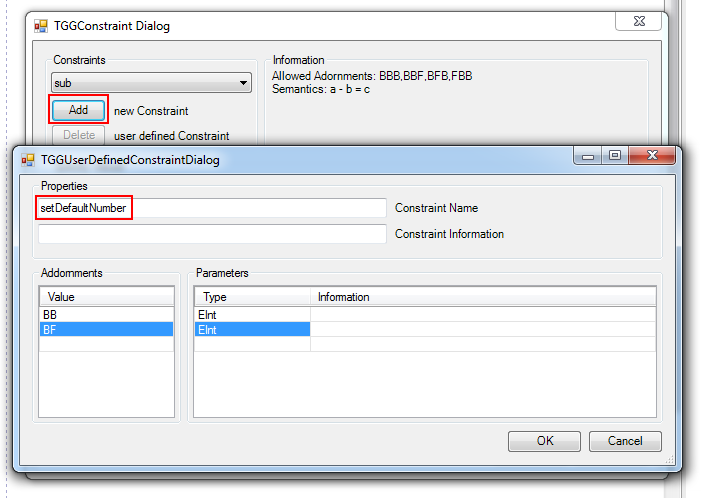
\includegraphics[width=\textwidth]{ea_SetDefaultNumberConstraint}
  \caption{Creating a custom constraint}
  \label{ea:setDefaultConstraintDialogue}
\end{center}
\end{figure}

\newpage

\item[$\blacktriangleright$] If successful, your diagram should be udpated with the changes as seen in Fig.~\ref{ea:ForAllEntryRuleUpdated}.

\vspace{0.5cm}

\begin{figure}[htp]
 \hspace{-2cm}
  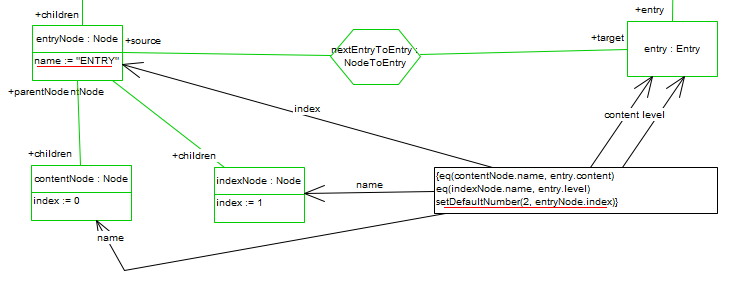
\includegraphics[width=1.4\textwidth]{ea_ForAllEntryRuleUpdated}
  \caption{New changes to \texttt{ForAllEntryRule}}
  \label{ea:ForAllEntryRuleUpdated}
\end{figure}

\vspace{0.5cm}

\item[$\blacktriangleright$] Save and validate your updated \texttt{DictionaryCodeAdapter}, but don't run the TGG -- we haven't included any
implementation for your constraint yet!

\jumpSingle{common cspConstraint}

\end{itemize}
